\documentclass[xcolor=pdftex,dvipsnames,table,mathserif]{beamer}
\usetheme{default}
%\usetheme{Darmstadt}
%\usepackage{times}
%\usefonttheme{structurebold}

\usepackage[english]{babel}
%\usepackage[table]{xcolor}
\usepackage{pgf,pgfarrows,pgfnodes,pgfautomata,pgfheaps}
\usepackage{amsmath,amssymb,setspace,centernot}
\usepackage[latin1]{inputenc}
\usepackage[T1]{fontenc}
\usepackage{relsize}
\usepackage{stmaryrd}
\usepackage{pdfpages}
\usepackage[absolute,overlay]{textpos} 


\newenvironment{reference}[2]{% 
  \begin{textblock*}{\textwidth}(#1,#2) 
      \footnotesize\it\bgroup\color{red!50!black}}{\egroup\end{textblock*}} 

\DeclareMathSizes{10}{10}{6}{6} 
\AtBeginSection[]{
  \begin{frame}
  \vfill
  \centering
  \begin{beamercolorbox}[sep=8pt,center,shadow=true,rounded=true]{title}
    \usebeamerfont{title}\insertsectionhead\par%
  \end{beamercolorbox}
  \vfill
  \end{frame}
}
\begin{document}
\title{Lecture 5: Pricing Equilibria and Mergers}
\author{Chris Conlon}
\institute{Grad IO}
\date{\today}

\frame{\titlepage}

\section{Antitrust and Mergers}

\begin{frame}
\frametitle{What is Antitrust?}
 \begin{itemize}
\item Debate: should we maximize \alert{efficiency/social surplus} or should we focus on \alert{consumer surplus}.
\begin{itemize}
\item US antitrust law focuses primarily on harm to consumers.
\item EC tends to also worry about harm to competing firms.
 \end{itemize}
 \item We know about DWL from market power from undergrad economics. However, without profits, why would firms innovate or perform R\&D?
 \begin{itemize}
\item Law understands this and awards temporarily monopolies via patents.
 \end{itemize}
\item Today, I am going to focus mostly on \alert{horizontal mergers} among competitors.
 \end{itemize}
\end{frame}

\begin{frame}
\frametitle{Antitrust Legislation : Sherman Act (1890)}
 \begin{description}
\item [Section 1]``Every contract, combination in the form of trust or otherwise, or conspiracy, in restraint of trade or commerce among the several States, or with foreign nations, is declared to be illegal'' (Violation involves an \alert{agreement}).
\item [Section 2] ``Every person who shall monopolize, or attempt to monopolize, or combine or conspire with any other person or persons, to monopolize any part of the trade or commerce among the several States, or with foreign nations, shall be deemed guilty of a felony''.
 \end{description}
 Three \textit{per se} violations
 \begin{itemize}
 \item (1) price fixing (2) horizontal market division (3) refusals to deal.
 \item Other violations are \textit{rule of reason}.
 \end{itemize}
 
\end{frame}

\begin{frame}
\frametitle{Antitrust Legislation : Clayton Act (1914)}
 \begin{description}
\item [Section 2] Prohibits some forms of price discrimination, but only when it lessens competition.
\item [Section 3] Prohibits sales based on the condition that the buyer not buy from your competitor (includes tying and exclusive dealing), but only when effect may be to substantially lessen competition.
\item [Section 7] Prohibits mergers where the effect of such acquisition may be substantially to lessen competition, or tend to create a monopoly in any line of commerce.
\item [Section 8] Prevents a person from being a director of multiple competing firms.
 \end{description}
\end{frame}

\begin{frame}
\frametitle{Antitrust Legislation : Hart-Scott-Rodino Act (1976)}
 \begin{itemize}
\item Required pre-notification and registration of large mergers
\begin{itemize}
\item Transaction: \$78.2 million
\item Size of Person: \$156.3 M with target of \$15.6 M or total transaction of \$312.6M
\item These are ``inflation adjusted'' each year.
\end{itemize}
\item Initial review period is 30 days after which DOJ/FTC can request additional information or allow merger to proceed.
\item Second review usually involves detailed information about  price-cost margins, market shares, etc. (Usually more info available than to academic researchers).
\item Can request information company would reasonably have (customer surveys, etc.).
\item After second review can ask for \alert{injunctive relief} or \alert{remedies} which merging parties can oppose in court.
 \end{itemize}
\end{frame}

\begin{frame}
\frametitle{DOJ/FTC Horizontal Merger Guidelines}
 \begin{itemize}
\item DOJ/FTC describe markets as:
\begin{itemize}
\item Highly Concentrated: $HHI \geq 2500$.
\item Moderately Concentrated: $HHI \in [1500,2500]$. $\Delta HHI \geq 250$ merits scrutiny.
\item Un-Concentrated: $HHI \leq 1500$.
\end{itemize}
\item Also consider \alert{unilateral effects}/UPP and \alert{coordinated effects}.
\item Three steps:
\begin{enumerate}
\item Market Definition
\item Measure Concentration/Initial Screening
\item Merger Simulation
\end{enumerate}
 \end{itemize}
\end{frame}

\begin{frame}
\frametitle{Step 1: Market Definition}
SSNIP
 \begin{itemize}
\item Small but significant and non-transitory increase in price (SSNIP): smallest relevant market where a hypothetical monopolist could impose a 5\% price increase. (For at least one year).
\item Under linear demand this amounts to a price cost margin and an elasticity (sometimes the \alert{critical elasticity}).
 \end{itemize}
 Tricky Examples:
  \begin{itemize}
\item Whole Foods vs. Wild Oats
\item Cellophane Fallacy.
 \end{itemize}
\end{frame}

\begin{frame}
\frametitle{Step 2: Concentration/Screening}
 \begin{itemize}
\item After we define the relevant market, compute the relevant HHI or UPP.
\item There can be both geographic and product market issues in the relevant market.
\item Some markets may be highly concentrated and others may not be.
\item Can ask for \alert{divestitures} as part of a \alert{remedy} if there are a few problematic markets in an otherwise uncontroversial merger.
 \end{itemize}
\end{frame}


\begin{frame}
\frametitle{Step 3: Merger Simulation}
 \begin{itemize}
\item Simulate the price effects of the merger
\item Take into account likely cost synergies (sometimes there are none).
\item Estimate post-merger prices and welfare.
 \end{itemize}
 This is what we will talk about next.
\end{frame}

\section{Merger Simulation}

\begin{frame}
\frametitle{Merger Simulation: Two Options}
 \begin{itemize}
\item Partial Merger Simulation
 \begin{itemize}
\item Simulate a new price for $p_j$ after acquiring good $k$ holding the prices of all other goods $(p_k,p_{-j})$ fixed.
\item Repeat for $p_k$ and all other products involved in the merger.
\item Compare price increases to \alert{synergies} or cost savings.
 \end{itemize}
 \item Full Merger Simulation
 \begin{itemize}
\item Write down the full system of post-merger FOC.
\item Adjust post-merger marginal costs for potential synergies.
\item Solve for all prices at the new (post-merger) equilibrium $(p_j,p_k,p_{-j})$.
 \end{itemize}
 \end{itemize}
\end{frame}

\begin{frame}
\frametitle{Differentiated Products Bertrand}
Recall the multi-product Bertrand FOCs:
\begin{eqnarray*}
\arg \max_{p \in \mathcal{J}_f} \pi_f (\mathbf{p}) &=& \sum_{j \in \mathcal{J}_f} (p_j - c_j) \cdot q_j(\mathbf{p}) \\
\rightarrow 0&=& q_j(\mathbf{p}) + \sum_{k \in \mathcal{J}_f} (p_k - c_k) \frac{\partial q_{k}}{\partial p_j}(\mathbf{p})
\end{eqnarray*}
It is helpful to define the matrix $\Omega$ with entries:
\begin{eqnarray*}
\Omega_{(j,k)}(\mathbf{p}) = \left\{\begin{array}{lr}
         - \frac{\partial q_{j}}{\partial p_k}(\mathbf{p}) & \text{for }  (j,k) \in \mathcal{J}_f\\
       	  \quad 0 & \text{for } (j,k) \notin \mathcal{J}_f
        \end{array} \right\}
\end{eqnarray*}
We can re-write the FOC in matrix form:
\begin{eqnarray*}
q(\mathbf{p}) = \Omega(\mathbf{p})\cdot(\mathbf{p}-\mathbf{mc})
\end{eqnarray*}
\end{frame}

\begin{frame}
\frametitle{Merger Simulation}
What does a merger do? \alert{change the ownership matrix}.
\begin{itemize}

\item Step 1: Recover marginal costs $\widehat{\mathbf{mc}} = \mathbf{p} +\Omega(\mathbf{p})^{-1}q(\mathbf{p})$.
\item Step 1a: (Possibly) adjust marginal cost $\widehat{\mathbf{mc}}\cdot (1-e)$ with some cost efficiency $e$.
\item Step 2: Change the ownership matrix $\Omega^{pre}(\mathbf{p}) \rightarrow \Omega^{post}(\mathbf{p})$.
\item Step 3: Solve for $\mathbf{p}^{post}$ via: $\mathbf{p} = \widehat{\mathbf{mc}} - \Omega(\mathbf{p})^{-1}q(\mathbf{p})$.
\end{itemize}
\pause
\vspace{0.5cm}
\begin{itemize}
\item The first step is easy (just a matrix inverse).
\item The second step is trivial.
\item The third step is tricky because we have to solve an implicit system of equations. $\mathbf{p}$ is on both sides.
\end{itemize}
\end{frame}




\begin{frame}{Solution Methods}
We were a bit vague on how we were solving the system of equations for $p^{post}$, the post-merger price.\\

\vspace{0.5cm}
General problem $F(x) = 0$ or $n$ nonlinear equations and $n$ unknowns $x = (x_1,\ldots, x_n) \in \mathbb{R}^n$.
\begin{eqnarray*}
F_1 (x_1,\ldots, x_n)  &=& 0 \\
F_2 (x_1,\ldots, x_n)  &=& 0\\
&\vdots&\\ 
F_{N-1} (x_1,\ldots, x_n)  &=& 0\\
F_N (x_1,\ldots, x_n)  &=& 0\\
\end{eqnarray*}
\end{frame} 

\begin{frame}{Solution Methods}
Helpful to write $F(x) = 0 \Leftrightarrow x - \alpha F(x) = x$ which yields the fixed point problem:
\begin{eqnarray*}
G(x) = x -\alpha F(x)
\end{eqnarray*}
Fixed point iteration
\begin{eqnarray*}
x^{k+1} = G(x^k)
\end{eqnarray*}
Nonlinear Richardson iteration or Picard iteration.\\
\vspace{0.5cm}
We need $G$ to be a \alert{contraction mapping} for iterative methods to guarantee a unique solution (often need strong monotonicity as well).
\end{frame} 

\begin{frame}{Gauss Jacobi: Simultaneous Best Reply}
Current iterate: $x^k = (x_1^k,x_2^k,\ldots,x_{n-1}^k,x_n^k)$.\\
\vspace{0.5cm}
Compute the next iterate $\alert{x^{k+1}}$ by solving one equation in one variable using only values from $x^k$ : 
\begin{eqnarray*}
F_1 (\alert{x_1^{k+1}},x_2^k \ldots, x_{n-1}^k, x_n^k)  &=& 0 \\
F_2  (x_1^k,\alert{x_2^{k+1}},\ldots,x_{n-1}^k,x_n^k)  &=& 0\\
&\vdots&\\ 
F_{n-1}  (x_1^k,x_2^k,\ldots,\alert{x_{n-1}^k},x_n^k)  &=& 0\\
F_n  (x_1^k,x_2^k,\ldots,x_{n-1}^k, \alert{x_n^k})  &=& 0\\
\end{eqnarray*}
Requires contraction and strong monotonicity.
\end{frame} 

\begin{frame}{Partial Merger Analysis}
\begin{itemize}
\item Hold all other prices $p_{-j}$ fixed at \alert{pre-merger} prices.
\item Adjust the marginal costs for potential efficiencies.
\item Consider only the FOC for product $j$
\begin{eqnarray*}
0&=& q_j(\mathbf{p}) + \sum_{k \in \mathcal{J}_f} (p_k - c_k) \frac{\partial q_{k}}{\partial p_j}(\mathbf{p})
\end{eqnarray*}
\item Solve for the new $p_j$ given the change in the products controlled by firm $f$: $\mathcal{J}_f \rightarrow \mathcal{J}_f'$
\item This is a single Gauss-Jacobi step (only products involved in merger).
\end{itemize}
\end{frame} 

\begin{frame}{Partial Merger Analysis: Why bother?}
\begin{itemize}
\item We only need own and cross elasticities for products involved in the merger.
\item Tends to show smaller price increases than full equilibrium merger analysis.
\item Only solving a single equation rather than a system of $J$ nonlinear equations.
\end{itemize}
\end{frame} 


\begin{frame}{Gauss Seidel: Iterated Best Response}
Current iterate: $x^k = (x_1^k,x_2^k,\ldots,x_{n-1}^k,x_n^k)$.\\
\vspace{0.5cm}
Compute the next iterate $\alert{x^{k+1}}$ by solving one equation in one variable updating as we go through:\begin{eqnarray*}
F_1 (\alert{x_1^{k+1}},x_2^k \ldots, x_{n-1}^k, x_n^k)  &=& 0 \\
F_2  (\alert{x_1^{k+1},x_2^{k+1}},\ldots,x_{n-1}^k,x_n^k)  &=& 0\\
&\vdots&\\ 
F_{n-1}  (\alert{x_1^{k+1},x_2^{k+1},\ldots,x_{n-1}^{k+1}},x_n^k)  &=& 0\\
F_n  (\alert{x_1^{k+1},x_2^{k+1},\ldots,x_{n-1}^{k+1}, x_n^{k+1}})  &=& 0\\
\end{eqnarray*}
Requires contraction and strong monotonicity.\\
You can speed things up (sometimes) by re-ordering equations.
\end{frame} 

\begin{frame}{Newton's Method}
\begin{enumerate}
\item Take an initial guess $x^0$
\item Take a Newton step by solving the following system of linear equations
\begin{eqnarray*}
J_F(x^k) s^k = - F(x^k)
\end{eqnarray*}
\item New guess $x^{k+1} = x^k + s^k$.
\item Good (Quadratic) Local convergence
\end{enumerate}
\begin{itemize}
\item Requires $J_F$ (Jacobian) to be Lipschitz continuous. 
\item Linearity means we do not need to take the inverse to solve the system (just QR decomp -- \texttt{backslash} in MATLAB).
\item Non-singularity of $J_F$ is weaker than strong monotonicity (more like PSD).
\end{itemize}
\end{frame} 

\begin{frame}{Fixed Point Iteration?}
\begin{itemize}
\item Can we iterate on the price relation until we converge to a new equilibrium?
\begin{eqnarray*}
\mathbf{p} \mapsfrom \widehat{\mathbf{mc}} - \Omega(\mathbf{p})^{-1}q(\mathbf{p})
\end{eqnarray*}
\item While tempting, this doesn't work. (It is \alert{not} a contraction).
\item There is a modification that is a contraction for logit type models.
\item You can always get lucky(!)
\end{itemize}
\end{frame}

\begin{frame}{Morrow Skerlos (2010) Fixed Point}
\begin{itemize}
\item For the logit (and variants) we can factor $\frac{\partial q_j}{\partial p_k}$ into two parts. 
\begin{eqnarray*}
\Omega_{jk}(\mathbf{p}) =  \underbrace{\alpha \cdot I[j=k] \cdot s_j(\mathbf{p})}_{\Lambda(\mathbf{p})} -  \underbrace{\alpha \cdot s_{j}(\mathbf{p}) s_{k}(\mathbf{p})}_{\Gamma(\mathbf{p})}
\end{eqnarray*}
\item $\Gamma(\mathbf{p})$ and $\Lambda(\mathbf{p})$ are $J \times J$ matrices and $\Lambda(\mathbf{p})$ is diagonal and $(j,k)$ is nonzero in $\Gamma(\mathbf{p})$ only if $(j,k)$ share an owner.
\item After factoring we can rescale by $\Lambda^{-1} (\mathbf{p})$
\begin{eqnarray*}
(\mathbf{p}-\mathbf{mc} ) \mapsfrom \Lambda^{-1}(\mathbf{p}) \cdot \Gamma(\mathbf{p})\cdot(\mathbf{p}- \mathbf{mc}) - \Lambda^{-1}(\mathbf{p})\cdot s(\mathbf{p})
\end{eqnarray*}
\item This alternative fixed point is in fact a contraction.
\item Moreover the rate of convergence is generally fast and stable (much more than Gauss-Seidel or Gauss-Jacobi).
\end{itemize}
\end{frame}


\section{Unilateral Effects}

\begin{frame}{What are Unilateral Effects?}
\begin{itemize}
\item In 2010 the Horizontal Merger Guidelines were updated to reflect a movement away from HHI/concentration based measures and \alert{Cournot} competition towards measures more in line with \alert{Differentiated Bertrand} competition.
\item Similar to partial merger analysis. Look at the incentives to raise prices for product $j$ before and after a merger, holding all other prices fixed.
\item Two key measures \alert{Upward Pricing Pressure} (UPP) and the primary input into UPP the \alert{Diversion Ratio}.
\item Intended for initial screening stage of merger evaluation, but sometimes substitute for full merger simulation.
\end{itemize}
\end{frame}

\begin{frame}
\frametitle{2010 Merger Guidelines}
\begin{quotation}
\textit{
In some cases, the Agencies may seek to quantify the extent of direct competition between a product sold by one merging firm and a second product sold by the other merging firm by estimating the diversion ratio from the first product to the second product. \alert{The diversion ratio is the fraction of unit sales lost by the first product due to an increase in its price that would be diverted to the second product. }Diversion ratios between products sold by one merging firm and products sold by the other merging firm can be very informative for \alert{assessing unilateral price effects, with higher diversion ratios indicating a greater likelihood of such effects}. Diversion ratios between products sold by merging firms and those sold by non-merging firms have at most secondary predictive value.}
\end{quotation}
\end{frame}

\begin{frame}
\frametitle{Unilateral Effects}
\begin{itemize}
\item Eliminating competition between the merging firms can itself constitute a substantial lessening of competition
\item Developed in the 1992 Guidelines, and larger role in the 2010 Guidelines
\item Based on modern theoretical literature: Farrell Shaprio (1990), Werden (1996), Farrel Shapiro (2010), Froeb and Werden (1998)
\item Extension to multiple products/firms may be tricky (Carlton 2010, Hausman, Moresei, Rainey (2010)).
\item Doesn't go as far as pass-through literature (Bulow Geanakoplos Klemperer (1985), Jaffe Weyl (2013)). 
\item Limited empirical results in academic literature: (Cheung 2013, Miller, Remer, Ryan, Sheu (2013), Conlon Mortimer (2013/5))
\item Possibly more empirical experience at DOJ/FTC.
\end{itemize} 
\end{frame}

\begin{frame}
\frametitle{What is the Diversion Ratio?}
\small
Ignore all but two merging products
\begin{block}{Pre-Merger}
Firm maximizes $\pi_j$ choosing $p_j$:
\begin{eqnarray*}
q_j(\mathbf{p^{(0)}}) + (p_j^{(0)} - c_j) \frac{\partial q_j(\mathbf{p^{(0)}})}{\partial p_j} &=& 0 
\end{eqnarray*}
\end{block}
\small
\begin{block}{Post-Merger}
Firm maximizes $\pi_j+\pi_k$ choosing $p_j$ only (with efficiency $e_j$):
\begin{eqnarray*}
q_j(\mathbf{p^{(1)}}) + (p_j^{(1)} - (1-e_j)\cdot c_j) \frac{\partial q_j(\mathbf{p^{(1)}})}{\partial p_j}  + (p_k^{(1)} - c_k) \frac{\partial q_k(\mathbf{p^{(1)}})}{\partial p_j}  &=& 0 \\
\end{eqnarray*}
\end{block}
\end{frame}

\begin{frame}
\frametitle{UPP Derivation}
\begin{block}{Difference between pre- and post- merger prices:}
Let $UPP_j \approx p_j^{1} -p_j^{0}$: 
\begin{eqnarray*}
UPP_j &\approx& (p_k -mc_k) \cdot \underbrace{\left[\frac{\partial q_j }{\partial p_j}\right]^{-1}  \left[\frac{\partial q_k }{\partial p_j} \right]}_{D_{jk}(\mathbf{p})} - E_j mc_j \\
GUPPI_j &=& D_{jk}(\mathbf{p}) \cdot  \frac{p_k - mc_k}{p_j} \\
\end{eqnarray*}
\end{block}
Leads some to state that diversion ratio $D_{jk}(\mathbf{p})$ is a sufficient statistic for unilateral merger effects.
\end{frame}

\begin{frame}
\frametitle{UPP Derivation : Multiple Products}
\begin{block}{Extension to multiple acquisitions:}
Very easy if we have that $p_j - mc_j = p - mc$ are the same for several values of $j$.  Then
\begin{eqnarray*}
UPP_j &\approx& (p - mc) \sum_k D_{jk}(\mathbf{p}) -  E_j mc_j \\
\end{eqnarray*}
\end{block}
If several brands of acquisition have the same markup -- can consider firm-level diversion. (We can aggregate diversion across similar flavors)
\end{frame}

\begin{frame}
\frametitle{Empirical Measures of Pricing Pressure}
\begin{description}
\item[Assumption] Proportional to market share?
\item[Price Cost Margins] Hart-Scott-Rodino Act/ Discovery/ provided by merging parties.
\item[Diversion as Data (Farrell Shapiro 2010)] \textit{The diversion ratio might be estimated using evidence generated in the merging firms' normal course of business. Firms often track diversion ratios in the form of who they are losing business to, or who they can win business from.}
\item[Diversion Surveys (Farrell Shapiro 2010)] \textit{Customer surveys can also illuminate diversion ratios, as can information about customer switching patterns.}
\item[Demand Estimation] If we can do this, can probably do full merger simulation. May depend on second-order information or parametric forms. Can also differentiate demand to get diversion.
\end{description}
\end{frame}

\begin{frame}
\frametitle{Experimental Interpretation (Conlon and Mortimer 2015)}
\begin{description}
\item[Population] All individuals who at current prices would buy $j$.
\item[Treatment] Not buying $j$.
\item[Outcome] Fraction who purchase $k$ instead.
\item[Instrument] $p_j$ functions as the instrument (it monotonically increases probability of treatment).
\item[Effect of Interest] treat only those individuals purchasing $j$ who are most price-sensitive. (ie: those who would leave  $j$ after a 5-10\% price increase).
\end{description}
\end{frame}

\begin{frame}{Diversion Experiments}
\begin{itemize}
\item Consider an experiment designed to measure diversion, where everything else is held fixed and $p_j$ is increased by $\Delta p_j$ 
\begin{eqnarray*}
\widehat{D_{jk}} &=& \left| \frac{\Delta Q_{k}}{\Delta Q_j} \right| =  \left| \frac{Q_{k}(\mathbf{p^{(1)}}) - Q_{k}(\mathbf{p^{(0)}})}{Q_{j}(\mathbf{p^{(1)}}) - Q_{j}(\mathbf{p^{(0)}})}   \right| = \frac{\int_{p_j^{0}}^{p_j^1}  \frac{\partial q_k(p_j,p_{-j})}{\partial p_j}\,\partial p_j }{\int_{p_j^{0}}^{p_j^1}   \frac{\partial q_j(p_j,p_{-j})}{\partial p_j} \, \partial p_j}
\end{eqnarray*}
\end{itemize}
\end{frame}

\begin{frame}{Diversion: Finite Price Change}
Think about the \alert{Local Average Treatment Effect}:
\begin{eqnarray*}
\widehat{ED_{jk} }&=& \frac{1}{\Delta q_j} \int_{p_j^{0}}^{p_j^{0}+\Delta p_j} \underbrace{\frac{\partial q_k}{\partial q_j}}_{D_{jk}(\mathbf{p})} \left| \frac{\partial q_j}{\partial p_j} \right|\, \partial p_j
\end{eqnarray*}
\begin{itemize}
\item Our estimated diversion measure is a weighted average of diversion, where the weights are the fraction of lost sales of $j$:  $w(\mathbf{p}) = \frac{1}{\Delta q_j} \frac{\partial q_j}{\partial p_j} (\mathbf{p})$
\item If demand declines quickly near the market price $ATE \approx D_{jk}(\mathbf{p})$ at $\mathbf{p}^{(0)}$.
\end{itemize}
\end{frame}

\begin{frame}
\frametitle{Thought Experiment -- Linear Demand for a Toyota Prius}
\begin{center}
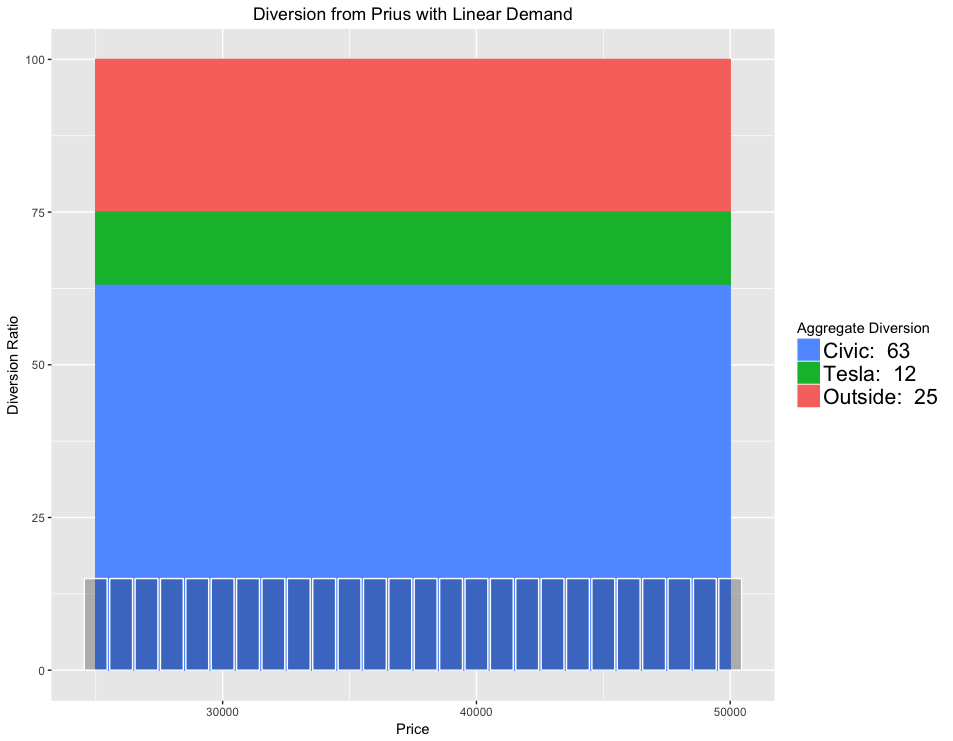
\includegraphics[width=4in]{./resources/new_prius_linear.png}
\end{center}
\end{frame}

\begin{frame}
\frametitle{Thought Experiment -- Inelastic CES Demand for a Prius}
\begin{center}
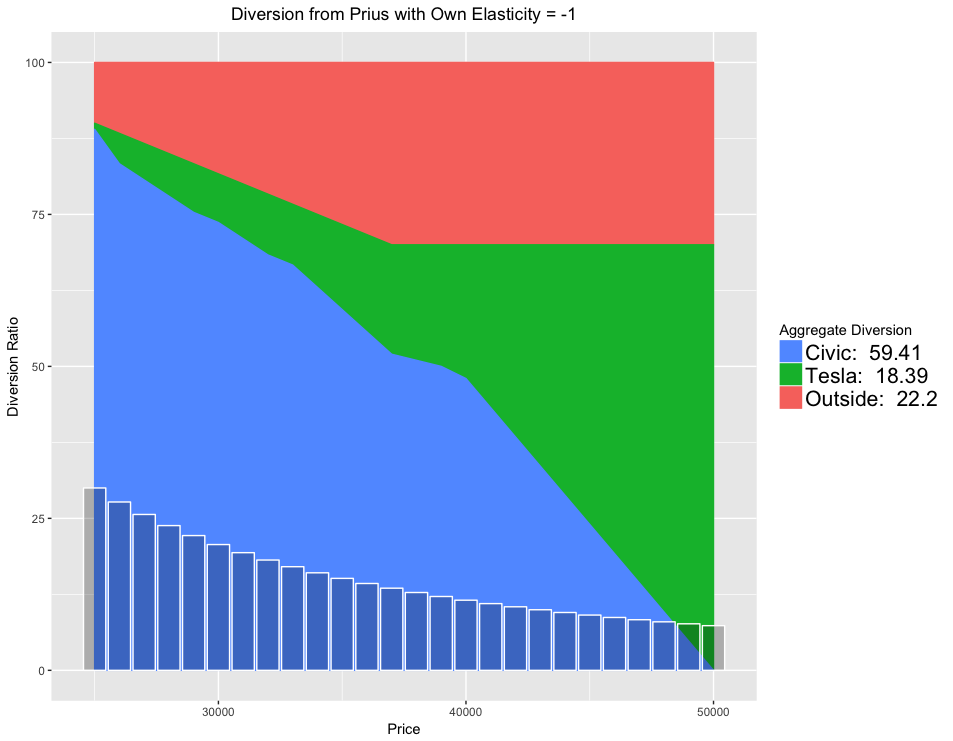
\includegraphics[width=4in]{./resources/new_prius1.png}
\end{center}
\end{frame}

\begin{frame}
\frametitle{Thought Experiment -- Elastic CES Demand for a Prius}
\begin{center}
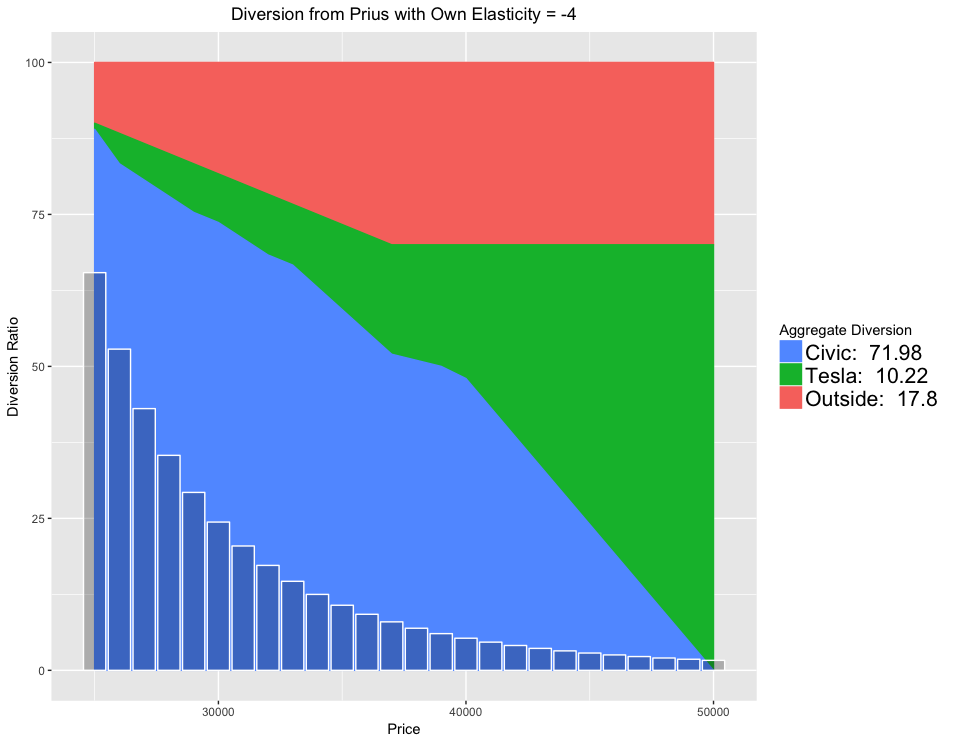
\includegraphics[width=4in]{./resources/new_prius4.png}
\end{center}
\end{frame}



\end{document}